\chapter{Choosing a projection}\label{ch:projection}

A flat map cannot keep every property of the globe. It can keep areas (equal-area), local shapes (conformal), or distances along some lines, but not all at once. Choose by what your map is used for.

\begin{figure}[H]\centering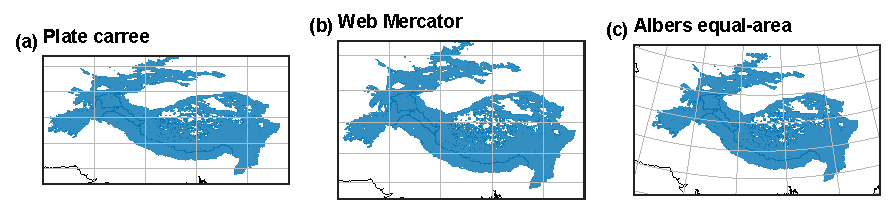
\includegraphics[width=\linewidth]{fig_projections.pdf}
\caption{The same region in three projections.}\end{figure}

\begin{tabularx}{\linewidth}{@{}lXl@{}}
\toprule
Your map & Good choice & Code \\
\midrule
Region at mid latitudes & Albers equal-area conic, with parallels at about a sixth and five-sixths of the height & \texttt{carto.albers(lon, lat1, lat2)} \\
A city or small area & The national grid or a UTM zone & \texttt{ccrs.OSGB()}, \texttt{ccrs.UTM(42)} \\
The world & Equal Earth, which keeps area & \texttt{ccrs.EqualEarth()} \\
Web tiles & Web Mercator, for navigation only & \texttt{ccrs.Mercator.GOOGLE} \\
\bottomrule
\end{tabularx}

\section{Never measure area in degrees}
A degree of longitude shrinks towards the poles, so any area taken from degrees is wrong. Table~\ref{tab:area} shows how far out each approach is, compared with Equal Earth, using the \texttt{shared-geodata} regions.

\begin{table}[H]\centering\footnotesize\caption{Area of two ranges by four routes.}\label{tab:area}\begin{tabular}{p{5.2cm}rrrr}
\toprule
How area is computed & Karakoram (km$^2$) & Error & Tian Shan (km$^2$) & Error \\
\midrule
Geographic degrees treated as flat{,} at the equator's scale & 91{,}702 & +23\% & 756{,}672 & +35\% \\
Web Mercator & 112{,}467 & +51\% & 1{,}022{,}497 & +83\% \\
Albers equal-area (ours) & 74{,}614 & +0\% & 560{,}184 & +0\% \\
Equal Earth & 74{,}614 & +0\% & 560{,}184 & +0\% \\
\bottomrule
\end{tabular}
\end{table}

Web Mercator inflates area most at high latitudes, which is why it should never be used for measuring. The routine is to reproject, and then measure:
\begin{lstlisting}[language=Python]
km2 = g.to_crs("ESRI:54034").area / 1e6      # cylindrical equal-area, in square metres
\end{lstlisting}

\section{Our helper}
\snippetcaption{research\_helpers/carto.py, albers(), lines 50--53}
\begin{lstlisting}[firstnumber=50]
def albers(central_lon, parallel_1, parallel_2, central_lat=None):
    """Equal-area conic, the usual choice for mid-latitude regions wider than they are tall."""
    lat = (parallel_1 + parallel_2) / 2 if central_lat is None else central_lat
    return ccrs.AlbersEqualArea(central_longitude=central_lon, central_latitude=lat, standard_parallels=(parallel_1, parallel_2))
\end{lstlisting}


\section{Scale bars and distortion}
A scale bar is only exactly true where a projection has no distortion: along the standard parallels of a conic map. On a small map of a large region, say this in the caption. On a world map, leave the bar out, since no single scale holds. \texttt{finish\_map()} accepts a sentence explaining why a map has no bar.
